\documentclass{article}

\usepackage[a4paper, left=1.5cm, right=1.5cm, top=2cm, bottom=2cm]{geometry}

\usepackage{../../../../components/components}

\usepackage{fancyhdr}
\usepackage{hyperref}
% Configuration des en-têtes et pieds de page
\pagestyle{fancy}
\fancyhf{} % reset tout

\fancyhead[L]{DL2 Math-Info PI4}
\fancyhead[C]{Projet informatique}
\fancyhead[R]{2025-2026}

\fancyfoot[L]{Ewen Rodrigues de Oliveira}
\fancyfoot[R]{\thepage}

\begin{document}

\docTitle{Rapport du projet : Symplexis (VR1a)}

\tableofcontents

\section{Introduction}

Symplexis résulte d'un constant : notre monde est un monde de conflits : géopolitiques comme économiques. C'est ce que Symplexis cherche humblement à simuler, en proposant un jeu de stratégie au tour par tour, dans lequel les joueurs incarnent des pays et doivent gérer leurs ressources, leur économie ainsi que lancer des attaques, jamais directement meurtrières, contre les autres joueurs.\\

Les actions sont simplifiées à des statistiques et des probabilités, pour que le jeu soit accessible à tous, tout en restant stratégique et amusant. Nous nous sommes inspirés de jeux de stratégie au tour par tour tels que Civilization, de serveurs PvP Faction sur Minecraft ou encore d'Age of Empire, tout en nourrissant le jeu de fonctionnalités malheureusement inspirées de l'actualité géopolitique.\\

L'équipe du projet est composée de cinq étudiants : Laurent CAI (MI2), Yaïr IFERGAN (MI2), Farzad RASHIDI (MI2), Ewen RODRIGUES DE OLIVEIRA (MI2), Stefan ZVONKOVSKI (INFO2).

\section{Conception du projet}
\subsection{Spécificités techniques}
Le projet n'utilise aucune librairie externe nécessaire au jeu en production. Toutefois, afin de faciliter le développement et en accord avec notre tuteur, le projet utilise \textbf{MAVEN} pour la gestion des dépendances et la compilation du projet.\\
Les dépendances sont uniquement à des fins de développement, pour assurer sa lisibilité et permettre l'exécution de tests unitaires.\\
\subsection{Architecture du projet}
Le projet suit les conventions imposées par Maven, avec une architecture en trois couches :
\begin{itemize}
    \item \textbf{Le modèle :} contient les classes représentant les entités du jeu (joueurs, cartes, attaques, etc.) et la logique métier du jeu (règles de combat, règles de déplacement, etc.).
    \item \textbf{La vue :} contient les classes responsables de l'affichage du jeu (interface graphique, affichage de la carte, etc.).
    \item \textbf{Le contrôleur :} contient les classes responsables de la gestion des interactions entre le modèle et la vue (gestion des événements, gestion de l'IA, etc.).
\end{itemize}

Pour s'abstraire de la complexité du monde réel, nous avons choisi de modéliser les pays du jeu à travers un graphe. Chaque pays est représenté par un nœud du graphe, et les routes entre les pays sont représentées par des arêtes du graphe.\\
Chaque noeud de ce graphe possède des propriétés : population, ressources, points d'action, etc. De même, lors d'attaques entre pays, les probabilités de succès sont calculées à partir de ces propriétés, ainsi que de la nature de l'attaque. Il est d'ailleurs possible de casser les routes entre les pays, ce qui rend les attaques plus difficiles, mais pas impossibles, grâce à des attaques de type "cyberattaque".

\subsection{Fonctionnalités principales}
Voici une liste non exhaustive des fonctionnalités principales du projet :
\begin{itemize}
    \item \textbf{IA de jeu :} Le joueur peut choisir de jouer contre une IA, qui est à la fois déterministe (elle choisit toujours la même action dans une même situation) et stochastique (nous l'avons plutôt nommée "adaptative" : elle ajuste les probabilités de ses actions en fonction de la situation de jeu, pour essayer d'optimiser ses chances de victoire).
    \item \textbf{Mode multijoueur :} le jeu peut être joué en multijoueur local, avec un système de tour par tour pour permettre à chaque joueur de jouer à son tour. La partie est lancée par un joueur-hôte, qui peut inviter d'autres joueurs à rejoindre la partie.
    \item \textbf{Système de métiers :} inspiré de serveurs PvP Faction sur Minecraft comme \href{https://nationsglory.fr}{NationsGlory} ou \href{https://paladium-pvp.fr}{Paladium}, les pays disposent de 4 métiers (agriculture, ingénierie, commerce et militaire), qui permettent de débloquer des fonctionnalités et d'améliorer les statistiques du pays. Par exemple, le métier d'agriculture permet d'augmenter la production de nourriture, le métier d'ingénierie permet de construire des routes, le métier de commerce d'avoir des réductions et le métier militaire permet d'améliorer les attaques.
    \item \textbf{Commerce 'void' :} afin de débloquer la partie et permettre la progression dans les métiers, les joueurs peuvent faire du commerce "void" : ils peuvent échanger des ressources et des points d'expérience contre de l'argent à une banque virtuelle, qui n'est pas un joueur du jeu. Cela permet aux joueurs de débloquer des fonctionnalités et de progresser dans les métiers, même s'ils ne sont pas en mesure de faire du commerce avec les autres joueurs.
    \item \textbf{Génération de la carte :} La carte est générée à partir d'un mélange d'automates cellulaires et de Perlin Noise, pour créer une carte réaliste et variée à chaque partie. Nous reviendrons là-dessus plus en détail lors de la soutenance.
    \item \textbf{Attaques :} Chaque joueur peut, selon son niveau militaire, lancer des attaques contre les autres joueurs, pour tenter de casser leurs routes, baisser la confiance qu'a leur population, etc.
\end{itemize}

\section{Progression du projet}
La répartition du ratio \textbf{lignes ajoutées + lignes supprimées} donne le graphique suivant, qui permet de visualiser la répartition du travail entre les membres de l'équipe :

\begin{center}
    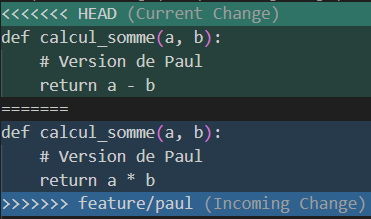
\includegraphics[width=0.5\textwidth]{./images/graph.png}
    \captionof{figure}{Répartition du travail entre les membres de l'équipe}
\end{center}

\attention{Il est important de noter que ce graphique ne reflète pas nécessairement la contribution de chaque membre de l'équipe, car certains membres peuvent avoir travaillé sur des tâches plus complexes qui ont nécessité moins de lignes de code, tandis que d'autres ont peut-être travaillé sur des tâches plus simples qui ont nécessité plus de lignes de code (notamment les interfaces graphiques).}

\subsection{Méthodologie de gestion de projet}
Comme demandé, le projet utilisait GitLab, avec une branche principale \texttt{main} et une branche de développement \texttt{dev}.\\
Chaque semaine, nous nous réunissions pour faire le point sur l'avancement du projet, identifier les tâches à faire pour la semaine suivante et répartir les tâches entre les membres de l'équipe.\\

\noindent Une pipeline a été mise en place pour gérer automatiquement les tests unitaires et la compilation du projet à chaque push sur la branche \texttt{dev}.\\

\noindent Afin de garantir la lisibilité du code, nous avons également utilisés les conventions Google Java Style Guide, avec l'aide de l'extension \textit{Checkstyle} sur Maven. Ainsi, le code est \textbf{intégralement documenté via des commentaires Javadoc}, qui peut être généré automatiquement pour produire une documentation complète du projet en version HTML.

\subsection{Étapes clefs}

\section{Problèmes rencontrés et solutions apportées}
\begin{itemize}
    \item \textbf{Problèmes de performance} : Arrivé à un certain moment, nous nous sommes rendu compte que le jeu devenait injouable (sur les machines tournant sous Linux, le jeu tournait sous moins de 10 \textit{FPS}). Nous avons identifié que le problème venait de l'affichage de la carte. Celle-ci était rendue à chaque tick, même si elle n'était pas modifiée, pixel par pixel.\\
    Nous avons résolu ce problème en implémentant un cache de la carte, via une \texttt{BufferedImage}, et réduit le nombre de fois où elle était mise à jour (seulement quand elle était modifiée et à la fin de chaque tour).
    \item \textbf{Optimisation de l'intelligence artificielle} : L'IA de notre projet souffrait de lourds problèmes d'optimisation. Elle utilisait systématiquement l'attaque la plus puissante, sans se soucier de son coût en points d'action.\\
    Pour palier à ce problème, nous avons entraîné une IA et lancé plusieurs milliers de parties (en accéléré, naturellement) pour collecter les données et trouver les meilleurs constantes pour les probabilités d'attaques, en fonction de la situation de jeu (nombre de points d'action restants, nourriture, etc.).\\\\
    L'IA n'est pas parfaite, nous avons tous les outils pour l'améliorer mais cela prendrait du temps, pour identifier les meilleurs constantes pour les probabilités d'attaques, en fonction de la situation de jeu (nombre de points d'action restants, nourriture, etc.). Nous avons déjà fait plusieurs étapes d'amélioration, qu'il conviendrait de continuer à faire pour améliorer l'IA.
\end{itemize}

\section{Axes d'amélioration}
À la fin du projet, nous avons identifié plusieurs axes d'amélioration qui seraient pertinents à implémenter pour améliorer le jeu :
\begin{itemize}
    \item \textbf{Amélioration de l'IA} : continuer les processus itératifs d'amélioration de l'IA, en collectant des données et en ajustant les constantes pour les probabilités d'attaques, en fonction de la situation de jeu,
    \item \textbf{Changer l'algorithme de création des routes} : la plupart des routes utilisent l'algorithme de Manhattan, qui est à notre niveau de Licence 2, mais qu'il serait intéressant de remplacer par un algorithme plus performant pour les rendre plus réalistes,
    \item \textbf{Système de sauvegarde :} implémenter un système de sauvegarde pour permettre aux joueurs de sauvegarder leur progression et de reprendre une partie plus tard.
\end{itemize}

\section{Crédits et remerciements}
Notre projet utilise certaines ressources externes afin d'améliorer l'expérience de jeu. Voici la liste exhaustive de ces ressources :
\begin{itemize}
    \item Drapeaux des pays : \href{https://www.reddit.com/r/vexillology/comments/svmfu6/i_created_a_bunch_of_flags_for_the_countries_in_a/}{r/vexillology}, IKEA
    \item Musique : \href{https://www.youtube.com/watch?v=Az6vUs2Cj1M}{Age of Empire III - Soundtrack}
    \item Pack d'icônes \textit{(source perdue)}
\end{itemize}

\noindent Un remerciement particulier à Vlady R. pour son accompagnement au long du projet, la qualité de ses conseils tant sur l'architecture que les algorithmes implémentés en jeu et la liberté laissée à l'équipe pour la réalisation du projet.

\end{document}